
\subsection{Symmetry constraints on nuclear NN forces}
When we come to the discussion of chiral effective field theory ($\chi$EFT) in a few lectures, we'll see that symmetry plays a central (if not THE central) role in building EFTs. Let us therefore start with a conventional discussion of general symmetry constraints on the NN Hamiltonian
as you would find in nuclear physics textbooks. Indeed, the approach outlined here was how people made progress Consider the NN potential as an operator that acts in the spin, isospin, and
position space Hilbert space.  That means that our building blocks are the Pauli matrics
for spin, $\sigmavec_i$, and isospin, $\taubold_i$, multiplied by functions of the 
spatial coordinates.

So we can specify the potential operator $\Vhat$ by giving all of the matrix elements
\beq
  \la \rvec'_1 s'_1 t'_1 \, \rvec'_2 s'_2 t'_2 | \Vhat | \rvec_1 s_1 t_1 \, \rvec_2 s_2 t_2 \ra
\eeq
where $s_i = \pm 1/2$ and $t_i = \pm 1/2$ are spin and isospin projections.
Suppressing spin and isospin for the moment, the action of $\Vhat$ on the coordinate
basis is
\beq
  \Vhat | \rvec_1 \rvec_2 \ra = \int V(\rvec'_1,\rvec'_2,\rvec_1,\rvec_2)|\rvec'_1 \rvec'_2 \ra
    d^3 r_1' \, d^3 r_2'  \;.
\eeq
The familiar local potential corresponds to the special
\beq
  V(\rvec'_1,\rvec'_2,\rvec_1,\rvec_2) = V(\rvec_1,\rvec_2)\delta(\rvec_1-\rvec'_1)\delta(\rvec_2-\rvec'_2)
   \quad \Longrightarrow \quad \Vhat | \rvec_1 \rvec_2 \ra = V(\rvec_1,\rvec_2)|\rvec_1\rvec_2\ra
   \;.
\eeq
This evidently has no dependence on the velocities of the particles, but just their positions.
It is not surprising then that we can translate the more general
non-locality into a velocity (or momentum 
dependence).  To do so, we first expand in a Taylor series the primed variables about
the unprimed ones:
\begin{align}
  |\rvec'_1 \rvec'_2 \ra &= | \rvec_1 \rvec_2 \ra +
  [(\rvec'_1 - \rvec_1) \dotvec \bm{\nabla}_1 + (\rvec'_2 - \rvec_2) \dotvec \bm{\nabla}_2]
  | \rvec_1 \rvec_2 \ra + \cdots
  \nonumber \\
  &= \ :\exp\left\{
    (\rvec'_1 - \rvec_1) \dotvec \bm{\nabla}_1 + (\rvec'_2 - \rvec_2) \dotvec \bm{\nabla}_2]
      \right\}: | \rvec_1 \rvec_2 \ra \;,
\end{align}
where the ``normal-ordering'' notation $:\Ohat:$ means here that the derivatives be moved
to act only to the right of the coordinates (and not on the coordinates).
Thus,
\begin{align}
 \Vhat | \rvec_1 \rvec_2 \ra &= \int V(\rvec'_1,\rvec'_2,\rvec_1,\rvec_2)
   \exp\left\{ 
   \frac{i}{\hbar} (\rvec'_1-\rvec_1)\dotvec\pvec_1 +
   \frac{i}{\hbar} (\rvec'_2-\rvec_2)\dotvec\pvec_2
     \right\}
 |\rvec_1 \rvec_2 \ra  d^3 r_1' \, d^3 r_2'
   \nonumber \\
  &= \widetilde V(\rvec_1,\pvec_1,\rvec_2,\pvec_2) | \rvec_1 \rvec_2 \ra \;.
\end{align}
So the general form is built from these operators, generally restricted to a low
order in momentum (quadratic), plus the allowed spin and isospin dependence.

But this is \emph{too} general a formulation: if we allow arbitrary dependence on
$\rvec_1,\pvec_1,\rvec_2,\pvec_2$ we will violate symmetries like spatial translation
invariance.  Similarly with possible structure for spin and isospin.  For example,
if we let $\sigma_0$ be the identity matrix, then since the $\sigma_i$, $i=0,1,2,3$ form
a complete basis in the spin space of one particle, a general expression for $\Vhat$
is 
\beq
   \Vhat = \sum_{i,j = 0}^{3} V_{ij} (\sigma_1)_i (\sigma_2)_j
    \;.
\eeq
So there are 16 $V_{ij}$ functions at this point.
Similarly for isospin.  But not every combination is consistent with the symmetries,
so in fact there are fewer.  What are they?



% If we're evaluating $U = e^{-i\bm{a\cdot P}}$ for translation by $\bm{a}$, we can use
% $\bm{P} = -i\bm{\nabla}$ and evaluate 
% $\la\rvec | e^{-i\bm{a\cdot P}} | \rvec'\ra = \delta^3(\rvec-\rvec')e^{-\bm{a\cdot\nabla_{\rvec'}}}$, being careful that the gradient acts correctly.  This
% achieves the translation.  However, it is generally easier to go to the eigenbasis of the
% symmetry generator (in this case momentum):
% \begin{align}
%   \la \rvec | e^{-i\bm{a\cdot P}} | \psi \ra
%   &= \int\!d^3k\, \la \rvec | e^{-i\bm{a\cdot P}} |\kvec\ra \la \kvec | \psi \ra \\
%   &= \int\!d^3k\,e^{-i\bm{a\cdot k}} \la \rvec |\kvec\ra \la \kvec | \psi \ra
%   = \int\!d^3k\, \frac{1}{(2\pi)^{3/2}} e^{i\bm{k\cdot(r-a)}} \la\kvec|\psi\ra
%   = \la \bm{r-a}|\psi\ra \;.
% \end{align}




\subsubsection{Operator structure of NN forces}


Let us step through the constraints on 
$\wt V(\rvec_1,\pvec_1,\sigvec1,\tauvec1,\rvec_2,\pvec_2,\sigvec2,\tauvec2)$
based on continuous space-time and discrete symmetries (but not yet chiral symmetry).
Generically when we use $\Vhat(1,2)$, the 1 and 2 refer to all of the indices.

\be

  \I $\Hhat = \That + \Vhat$ is hermitian and so is $\That$, therefore $\Vhat$ is hermitian.

  \I For identical particles, invariance under interchange of coordinates: $V(1,2) = V(2,1)$.
  This is connected to the symmetry of the two-particle wave function $|1\, 2\ra$.
  %[\emph{Add a specific case; check F+W.}]

  \I Translational invariance in space.  The unitary transformation for translations 
  by $\bm{a}$ is
  \beq
     U = e^{-i \bm{a\cdot P}}  \;,
  \eeq
  where $\bm{P}$ is the total center-of-mass momentum (the generator of translations).
  It results in
  \beq
    \rvec'_i = \rvec_i - \avec \;, \quad \kvec'_i = \kvec_i \;, \quad
      \sigvec{i}' = \sigvec{i} \;, \quad \taubold_i' = \taubold_i \;.
  \eeq
  Therefore we require 
  \beq
     [\bm{P},\Vhat] = 0 \;.
  \eeq
  In the full coordinate-space form (suppressing spin and isospin), 
  \beq
    \la \rvec_1\ \rvec_2 | \Vhat | \rvec'_1\ \rvec'_2 \ra
    =    \la \rvec_1-\avec\ \rvec_2-\avec | \Vhat | \rvec'_1-\avec\ \rvec'_2-\avec \ra
    \quad \Longrightarrow \quad \la \rvec_1-\rvec_2 | \Vhat | \rvec'_1-\rvec'_2 \ra
    = \la \rvec | \Vhat | \rvec' \ra
    \;.
  \eeq
  For $\wt V$ this means
  \beq
    V(1,2) = \wt V(\rvec,\pvec_1,\sigvec1,\tauvec1,\pvec_2,\sigvec2,\tauvec2)
      \;.
  \eeq

  % \I Translational invariance in time $\Longrightarrow$ $\Vhat$ is time independent.
  % [\emph{Does this really follow?  Translational invariance in space doesn't mean
  % it is space independent.  And why can't we have a time dependent (e.g., external)
  % potential?  Ok, the NN one isn't, but isn't this related to energy dependence?
  % Or the definition of a potential. Punt on this I think!}]

  \I Galilean invariance (more generally Lorentz invariance).
  Nuclear low-lying states have $|\pvec| \sim 200\,$MeV, so $p/m \approx 0.2$
  and $(v/c)^2 < 0.1$.  This is small but not \emph{negligible}, which suggests
  we should treat it as a $1/m$ expansion.
  Galilean invariance says that the physics looks the same from a moving frame,
  so $\rvec'_i = \rvec_i$, $\pvec'_i = \pvec_i - m_i\bm{u}$, $\sigvec{i}' = \sigvec{i}$,
  $\tauvec{i}' = \tauvec{i}$.  The unitary operator is (total mass $M$ and
  center-of-mass position operator $\bm {R}$):
  \beq
     U = e^{-iM\bm{u\cdot R}} \;, \quad \mbox{where } \quad M = \sum_i m_i 
     \quad\mbox{and}\quad \bm{R} = \frac{1}{M}\sum_i m_i \rvec_i \;.
  \eeq

This results in
  \beq
    V(1,2) = \wt V(\rvec,\pvec,\sigvec1,\tauvec1,\sigvec2,\tauvec2)
    \;.
  \eeq

  \I Rotational invariance requires $[\bm{J},V] = 0$, where is the \emph{total}
  angular momentum, i.e., $\bm{J} = \bm{L} + \bm{S}$.
  There are three independent scalars from $\rvec$ and $\pvec$, namely
  $\rvec^2$, $\pvec^2$, and $\rvec\dotvec\pvec + \pvec\dotvec\rvec$.
  The latter must appear quadratically because of time-reversal invariance (below),
  and it is more convenient to use $\bm{L}^2 = (\rvec\times\pvec)^2$.  The only
  vector to combine with a linear appearance of $\bm{S}$ is $\bm{L}$ to make 
  a spin-orbit interaction.
  There are only limited choices (see Okubo and Marshak, Ann.\ Phys.\ {\bf 4}, 166
  (1968) for full details).

 \I Parity $P$ is space reflection, which has the effect:
  \beq
    \rvec'_i = -\rvec_i\;, \quad \kvec'_i = -\kvec \;, \quad
      \sigvec{i}' = \sigvec{i} \;, \quad \taubold_i' = \taubold_i \;.
  \eeq
If we perform two space reflections we are back where we started, so
$P^2 = 1$ and the eigenvalues are $\pm 1$.
Parity is conserved by the strong interaction but
violated by the weak interactions; however, the parity-violating matrix elements
are small (of order $\sim0.1\,$eV).  This violation
was first observed in the beta decay of polarized $^{60}$Co
by Wu et al. in 1957, where the polarization of the nuclear spin defines a direction and
a preferential emission of electrons in the opposite direction of the spin was observed.


 \I Time reversal $T$ has the effect: 
  \beq
    \rvec'_i = \rvec_i\;, \quad \kvec'_i = -\kvec \;, \quad
      \sigvec{i}' = -\sigvec{i} \;, \quad \taubold_i' = \taubold_i \;.
  \eeq
  $T$ is violated in the standard model [from indirect CP violation in $K^0$ decay].
  $C$ exchanges particles and antiparticles.  There are active
  direct searches for $T$ violation by looking for permanent dipole
  moments in neutrons, nuclei,  and atoms.

  \I Baryon and lepton number conservation.
  $B$ violated by weak interactions.  $L$ would be violated if
  neutrinos are Majorana, which means they are their own antiparticles.

 \I Isospin charge symmetry.
    $p\leftrightarrow n$ and 

    Charge independence.  Scattering length for \Ssinglet: 
    \beq
      a_{nn} \approx (a_{pp}- \mbox{Coulomb}) \approx -18\,\mbox{fm} 
    \eeq 
    which is isospin charge symmetry.  But $a_{np} \approx -23.7\,$fm, which shows that
    charge independence breaking is stronger.
    Both are broken by Coulomb and other e/m plus $m_u \neq m_d$ effects.
\ee

In the end, the constraints lead to
\beq
  V_{NN} = V_1(\rvec,\pvec,\sigvec1,\sigvec2) 
    + V_\tau(\rvec,\pvec,\sigvec1,\sigvec2)) \tauvec1\dotvec\tauvec2
\eeq
where we have explicitly applied translational and rotational invariance to write these
in terms of $\rvec$ and $\pvec$ (remember that these are operators).
We further classify $V_1$ and $V_\tau$ into
central (scalar), vector (spin-orbit),
and tensor, with spin structures of rank 0,1,2:
\begin{itemize}
  \I \textbf{central parts:}
   \beq
      V_1(\rvec,\pvec) + V_\sigma(\rvec,\pvec)\, \sigmavec_1\dotvec\sigmavec_2 
      \;,
   \eeq

   \I \textbf{vector parts:}
   \beq
     V_{LS}(\rvec,\pvec) {\bm L\cdot S} \;,
   \eeq

   \I \textbf{tensor parts:}
   \beq
     V_{T}(\rvec,\pvec) S_{12}(\rhat)
   \eeq
   with tensor operator
   \beq
     S_{12}(\rhat) \equiv \rhat\bm{\cdot\sigma_1} \rhat\bm{\cdot\sigma_2}
       - \frac13 \sigmavec_1\dotvec\sigmavec_2 
   \eeq
   [\emph{Quick question: Why do we subtract off the 2nd term?}]

\end{itemize}
The full operator form in coordinate space is:
\beq
\left\{
  \rm{1}_{\rm spin},\, \sigmavec_1\dotvec\sigmavec_2,\, S_{12}(\rhat),\,
   S_{12}(\phatbold),\, \bm{L\cdot S},\, (\bm{L\cdot S})^2
\right\} \times \left\{\bm{1}_{\rm isospin}, \tauvec1\dotvec\tauvec2
\right\}
\;,
\eeq
times scalar operator-like functions of $r^2$, $p^2$, and $L^2$ (rather than
$\rvec\dotvec\pvec$).
In momentum space, the full operator form is:
\beq
\left\{
  \rm{1}_{\rm spin},\, \sigmavec_1\dotvec\sigmavec_2,\, S_{12}(\qhatbold),\,
   S_{12}(\khatbold),\, i\bf{S\cdot(q\times k),\, 
   \sigmavec_1\bm{\cdot (q\times k)}\, \sigmavec_2\bm{\cdot (q\times k)}}
\right\} \times \left\{\bm{1}_{\rm isospin}, \tauvec1\dotvec\tauvec2\right\}
\;,
\eeq
where $\qvec\equiv \pvec'-\pvec$ and $\kvec\equiv(\pvec'+\pvec)/2$, times
scalar functions of $p^2$, $p'{}^2$, and $\pvec\dotvec\pvec'$.





\subsection{Motivation and background for EFT}

  \subsubsection{Problems with phenomenological potentials}
  
   The best potential models (such as AV18) can describe with $\chi^2/\mbox{dof}
    \approx 1$ all of the NN data (about 6000 points) below the
    pion production threshold.  So what more do we need?  
  Some limitations of these potentials:
   \bi
    \I They usually have a very strong repulsive short-range part
     that requires special (non-systematic) treatment in 
     (some types of) many-body calculations of nuclear structure.
     
     \I It is difficult to estimate the theoretical error in a calculation
       and the range of applicability (i.e., where should it fail?).
     
     \I Three-nucleon forces (3NF) are largely included as
     under-constrained and non-systematic models.  How can we define 
     \emph{consistent} 3NF's
     and operators (e.g., including-meson exchange currents)?
     
     \I Models are largely unconnected to QCD (e.g., chiral
     symmetry is only respected in part).  They don't connect
     NN and other strongly interacting processes (e.g., $\pi\pi$
     and $\pi N$).  
%     
     Lattice QCD will be able to predict NN, 3N observables for 
     high pion masses.  How can we extrapolate to physical pion masses?
   %  How to make use of the results for more complex systems? 

   \ei
   To address these limitations, we seek a systematic alternative: effective (field) theory. Before getting into the nitty gritty details, let's start with some boilerplate about the general philosophy of low energy effective theories.
    

  \subsubsection{Effective theories: Appeal to authority :)}

Here we pull some nice quotes from H. Georgi, 
Ann.\ Rev.\ Nucl.\ Part.\ Sci. \textbf{43}, 209 (1993). [Note: while Georgi has some nice qualitative discussions in the intro, the bulk of the review article is at a pretty high level and assumes a solid QFT background.  Perhaps the best introductory treatment that does not require the heavy machinery of QFT is the lecture notes by Peter Lepage entitled ``How to Renormalize the Schr\"odinger Equation", which can be found on the course website. ]

Some relevant quotes from Georgi about effective theories: 
 \bi
 \I \emph{
  {\re One of the most astonishing things about the world in which we live is that there seems to be interesting physics at all scales.}}
  \I \emph{
  To do physics amid this remarkable richness, it is convenient to be able to isolate a set of phenomena from all the rest, so that we can describe it without having to understand everything.
  Fortunately, this is often possible. We can divide up the parameter space of the world into different regions, in each of which there is a different appropriate description of the important physics. {\re Such an appropriate
  description of the important physics is an ``effective theory.''}}
  \I \emph{
  The common idea is that if there are parameters that are very large or very small compared to the physical quantities (with the same dimension) that we are interested in, 
  {\re we may get a simpler approximate description of the physics by setting the small parameters to zero and the large parameters to infinity.} Then the finite effects of the parameters can be included as small perturbations about this simple approximate starting point.}  
 \ei

Any time there is a hierarchy of (separated) energy scales, think EFT!   Even if coupling constants are large (i.e., strongly interacting), the existence of a well-separated hierarchy of scales suggests a small parameter to expand in (i.e. ,the ratio of the low- and high-energy scales).


Examples from our physics experiences and this program of such effective theories (you give more!):
  \bi
 \I non-relativistic quantum (or classical) mechanics: $c\rightarrow \infty$;

 \I size of a charge distribution $\rightarrow 0$ (multipole expansion);

 \I mass of the proton in a hydrogen atom $\rightarrow \infty$;

 \I asphericity of a cow $\rightarrow 0$;

 \I number of colors in QCD $\rightarrow\infty$;

 \I  chiral effective \emph{field} theory (EFT): $m_\pi \rightarrow 0$, $M_N \rightarrow \infty$.
  \ei
\noindent
You add some!

 \subsubsection{Principles of low-energy effective theories}


  \begin{figure}[tbh]
  \begin{center}
    \includegraphics[width=2.in]{figures/resol3}~~~%
    \includegraphics[width=2.in]{figures/resol3a}~~~%
    \includegraphics[width=2.in]{figures/resol3b}
    \caption{Left: high-resolution, with wavelength of probe short compared
    to characteristic size of probed structure.  Middle: low-resolution probe
    doesn't resolve the details (because of diffracton).  Right: low-energy
    theory takes advantage and replaces short-distance with long-distance
    degrees of freedom.}
    \label{fig:resolving}
  \end{center}
  \end{figure}

Summary of the basic principles:
\bi
 \I
 If system is probed at low energies,
     fine details are not resolved.
 \I So we can use low-energy variables for low-energy processes
        (as they can be easier, more efficient, \ldots).
 \I The short-distance structure can be 
        \emph{replaced} by something simpler  
         (and wrong at short distances!) 
        without distorting low-energy  observables.  It is important that being
        wrong at short distances (``incorrect UV behavior'') doesn't matter but also
        cautions us that when it works for long distances, we should not conclude
        that we know about the UV.
  \I This is systematically achieved by the
         effective field theory.
\ei

There are some basic physics principles underlying any low-energy
    effective model or theory.
A high-energy, short-wavelength probes sees details.  E.g.,
  electron scattering at Jefferson Lab resolves the quark substructure
  of protons and neutrons in a nucleus. 
But at lower energies, details are not resolved,
  and one can replace short distance structure, as in
  a multipole expansion of a complicated charge or current distribution.
  So it is not necessary to do full QCD.
It is not obvious that this will work in quantum mechanics as
  it does for pixels or point dots or the classical multipole expansion,
  because \emph{virtual} states can have high energies that are not, in
  reality, simple.  Renormalization theory says it can be done!  (More
  later!)  It doesn't say that we are \emph{insensitive} to all short-distance
  details, only that there effects at low energies
   can be accounted for in a simple way.
Effective \emph{field} theory is a systematic approach to carrying out
  this program using a local field theoretical Lagrangian framework.  

 
%\bibliography{srg_refs}

To begin, we want to apply these ideas to the simplest possible example, for which
the resolution is so low we don't resolve \emph{any} interaction between
the particles.  For the nuclear case, this means that the exchange of pions
is considered short-ranged; that is the pion is a heavy degree of freedom
that is replaced (as are all other interactions) by contact interactions.

First, we'll lay out the basic ideas of renormalization and power
counting for the simplest case: a natural scattering length.  After that, the more interesting case for nuclear physics of an unnatural scattering
length will be explored in detail.


\subsection{Pionless effective field theory}

\subsubsection{Low-energy simplication of boson exchange interactions}

%\subsection{Origin of contact forces from meson exchange}


  \begin{figure}[tbh]
  \begin{center}
    \includegraphics[width=3.8in]{figures/force_ranges}
    \caption{Ranges associated with boson exchange.  The intermediate
    two-pion exchange attraction can be simulated with isoscalar, scalar
    exchange (``$\sigma$'').}
    \label{fig:obe_ranges}
  \end{center}
  \end{figure}

Let's first get some intuition about what NN forces would look like
at low-energies.  For this purpose, it is instructive to start with
boson exchange potentials.
Consider Fourier transforming to momentum space
a Yukawa potential with mass $\mu$ arising from one of the
boson exchanges considered in the last lecture
(without paying attention to the overall normalization), 
 \beq
   g^2\frac{e^{-\mu |{\bf r}|}}{4\pi|{\bf r}|} \longleftrightarrow
           \frac{g^2}{({\bf k'} - {\bf k})^2 + \mu^2} \;,
           \label{eq:FT_Yukawa}
 \eeq          
which manifestly
depends on ${\bf k}^2$, ${\bf k'}{}^2$, and $\bm{k\cdot k'}$.
(Note: we are ignoring any spin or isospin structure here.)
Now suppose we are at very low resolution, which means low momenta    
$k,k' \ll \mu$ (the deBroglie wavelengths are long).
We can Taylor expand in Eq.~\eqref{eq:FT_Yukawa}: 
\beq
  A_0 + A_2({\bf k}^2+ {\bf k'}{}^2) + A_2' {\bf
      k}\cdot {\bf k'} + \cdots 
\eeq  
%
These terms are called \emph{contact interactions} because when Fourier transformed to
coordinate space they become delta functions in the interparticle distance 
and derivatives of such delta functions:
\beq
   \la \kvec | A_0 | \kvec' \ra \propto A_0 \int\! d^3x\,
     e^{i\kvec\cdot\xvec} e^{-i\kvec'\cdot\xvec}
     = A_0 (2\pi^3)\delta(\xvec) \;.
\eeq
So this implies that at low resolution we can replace an extended interaction
(in this case, from the exchange of a particle) with a series of contact interactions.

If all we ever did was first-order perturbation theory, then a simple Taylor expansion
like this is all we need and we could pick the $A_i$'s to match the corresponding
Taylor expansion of the Yukawa term-by-term to reproduce the results of
the Yukawa theory.  
But what if we do second-order perturbation theory (or include the effects of
all orders by solving the Schr\"odinger equation)?
Then the sums over intermediate states become integrals over the momenta,
which then
contain parts where 
for which $k,k' \geq \mu$ and the expansion does not apply (i.e., it is
wrong at high energies).
What do we do? Stay tuned!


\subsubsection{Recap of effective range expansion}

Because we are considering the low-energy limit of a theory, we expect
we will reproduce the physics of the effective range expansion briefly discussed in Morten's lectures. 
This is generically called the ``pionless'' EFT,  because there are \emph{no} 
long-range degrees of freedom (i.e., the pion is treated as heavy rather than almost massless!)

%
Recall that the partial wave expansion of the scattering amplitude or
the on-shell $T$-matrix (which is only different by a multiplicative factor) takes
the form
\beq
  f(k,\theta) \equiv \frac{m}{4\pi}T(k,\cos\theta) = \sum_{k=0}^\infty
   \frac{2l+1}{k\cot\delta_l(k) - ik}  P_l(\cos\theta)
   \;.
\eeq


As first shown by Schwinger, $k^{2l+1}\cot\delta_l(k)$
has a power series expansion in $k^2$ (see Newton for more details on proving this).  
The radius of convergence is dictated by how the potential falls off for large $r$;
for a Yukawa potential of mass $m$, this radius is $m/2$.
For $l=0$ the expansion is
 \beq
   k\cot\delta_0(k) = -\frac{1}{\re a_0} + \frac12 {\bl r_0} k^2
      - Pr_0^3 k^4 + \cdots \;,
 \eeq
which defines the $S$-wave \emph{scattering length} $a_0$, the $S$-wave
\emph{effective range} $r_0$ and the 
$S$-wave shape parameter $P$ (often these are written $a_s$ and $r_s$ or
$a$ and $r_e$).
Note the sign conventions.
For $l=1$ the convention is to write
\beq
  k^3 \cot \delta_1(k) = -\frac{3}{a_p^3} \;,
\eeq
which defines the $P$-wave scattering length $a_p$ (with dimensions of a length).

The effective range expansion for hard-sphere scattering (radius $R$) is
(just do the Taylor expansion with $\delta_0(k) = -kR$):
 \beq
  k \cot(-kR) = -\frac{1}{R} + \frac13 R k^2 + \cdots
      \quad \Longrightarrow \quad
      a_0 = R\, \quad r_0 = 2R/3
 \eeq
(note the sign of $a_0$) so the magnitudes of the
effective range parameters are all the order 
the range of the interaction $R$.  
The radius of convergence here is infinite because the potential is identically
zero beyond some radius.  

For more general cases, we find that
while $r_0 \sim R$, the range of the potential, $a_0$ can be
anything:
\bi
  \I if $a_0 \sim R$, it is called ``natural'';
  \I $|a_0| \gg R$ (unnatural) is particularly interesting,
   e.g., for neutrons or cold atoms.
\ei
We can associate the sign and size of $a_0$ with the behavior of the scattering wave
function as the energy (or $k$) goes to zero, since
\beq
    \frac{\sin(kr + \delta_0(k))}{k} \underset{k\rightarrow 0}{\longrightarrow} r-a_0
    \;,
\eeq
so in the asymptotic region the wave function is a straight line with intercept $a_0$
(see Fig.~\ref{fig:scattering_length_figures}). We see that 
$a_0$ ranges from $-\infty$ to $+\infty$ (are there excluded regions?).

  \begin{figure}[tbh]
  \begin{center}
    \includegraphics[width=2.8in]{figures/scattering_length_positive.png}~~~~~%
    \raisebox{.08in}{\includegraphics[width=3.1in]{figures/scattering_length_negative.png}}
    \caption{Identifying the $S$-wave scattering length $a_0$ by looking at
    $k\rightarrow 0$ wave functions. [credit to ???]}
    \label{fig:scattering_length_figures}
  \end{center}
  \end{figure}

Let us consider the case of low-energy scattering for $l=0$.  Then the $S$-wave scattering 
amplitude is (recall Eq.~\eqref{eq:fl_def}) 
\beq
   f_0(k) =  \frac{1}{-1/a_0 - ik}  
      \qquad \Longrightarrow  \qquad
      \sigma(k) = \frac{4\pi}{1/a_0^2 + k^2} \;.
   \label{eq:f0_ere}
\eeq 
In the natural case, $|ka_0| \ll 1$ and $f_0(k)\rightarrow -a_0$ at low $k$ and
\beq
    \frac{d\sigma}{d\Omega} = a_0^2 \qquad \Longrightarrow \qquad \sigma = 4\pi a_0^2
    \;.
\eeq
Also, $\delta_0(k) \approx -ka_0$ implies that the sign of $a$ corresponds to the sign of $V$
(if strictly attractive or repulsive).
Figure~\ref{fig:scattering_length_figures} tells us that to get large $a_0$ (unnatural),
we need to have close to a zero-energy bound state (so the wave function is close to
horizontal in the asymptotic region).  
If $a_0>0$, we have a shallow  bound state (i.e., close to zero binding energy) 
while if $a_0<0$ we have a nearly bound (virtual)
state.
%
The limit of $|a_0| \rightarrow \infty$ is called the unitary limit; the cross section
becomes
\beq
   \frac{d\sigma}{d\Omega} \longrightarrow \frac{1}{k^2}
   \qquad \Longrightarrow \qquad \sigma = \frac{4\pi}{k^2}
   \;,
\eeq
which is the largest it can be consistent with the constraint of unitarity.



Schwinger first derived the effective range expansion (ERE) back in
  the 1940's and then Bethe showed an easy way to derive (and
  understand) it.  This is apparently a common pattern with Schwinger's work!
The implicit assumption here is that the potential is
  short-ranged; that is, it falls off sufficiently rapidly with
  distance.  This is certainly satisfied by any potential that actually
  vanishes beyond a certain distance.  Long-range potentials like the
  Coulomb potential must be treated differently (but a Yukawa potential, which
  has a finite range although non-vanishing out to $r \rightarrow\infty$, is ok).

When first identified, the ERE was a disappointment because it meant that scattering
experiments at low energy could not reveal the structure of the potential.  
For example, it is impossible to invert the expansion at any finite order to find a potential that
correctly gives scattering at higher energies.
All you determined were a couple of numbers (scattering length and effective range) and any
potential whose ERE was fit to these would reproduce experimental cross sections.     

In the modern view we are delighted with this:  the low-energy theory is determined
by a small number of constants that encapsulate the limited high-energy features 
that affect the low-energy physics (in many ways like a multipole expansion).
We can devise an effective theory (called the ``pionless effective theory'')
to reproduce the ERE and consistently extend it to include the coupling to external probes
(and other physics). Here we first consider how to reproduce this result in the natural case $a_0\sim R$; the more interesting (and relevant for nuclear physics!) unnaturally large scattering length case $|a_0| >> R$ will be looked at after that. 



\subsubsection{In search of a perturbative expansion}

If $a_0$ is {natural}, then low-energy scattering simplifies further.
Let's take the hard sphere potential as a concrete example.
The ERE in this case is indeed natural (recall that $\delta(k) = - kR$):
\beq
    k\cot(-kR) = -\frac{1}{a_0} + \frac12 r_0 k^2 + \cdots
     = -\frac{1}{R} \Bigl[
       1 - \frac{(kR)^2}{3} - \frac{(kR)^4}{45} + \cdots
       \Bigr] \;,
\eeq
and so if $kR$ is small, we have a convergent expansion.
This means that the scattering amplitude itself also
has a perturbative expansion in $k$:
\begin{align}
  {f_0(k)} &= \frac{1}{k\cot\delta(k) - ik}
  = \frac{1}{-\frac{1}{a_0} + \frac12 {r_0} k^2 + \cdots - ik}
  = \frac{-a_0}{1 - \frac12 a_0 r_0 k^2 + \cdots + ia_0 k}
  \nonumber \\ 
    & \longrightarrow -a_0 \bigl[ 1 - ia_0 {\re k} - (a_0^2 - a_0 r_0/2)
              {\re k^2} + {\cal O}({\re k^3} a_0^3) \bigr]
  \nonumber \\ 
          & \longrightarrow -R[1 - ikR - 2k^2 R^2/3 + {\cal O}(k^3R^3)] \;,
          \label{eq:f0_pert}
\end{align}
where in the last line we substituted the particular case of hard-sphere
scattering.
That is, for scattering at momentum $k \ll 1/R$, 
we should recover a perturbative expansion in $kR$ for the scattering amplitude
(because $a_0$ and $r_0$ are of order $R$),
or more generally, where we leave the coefficients of the expansion free.
%
Note that the perturbative expansion is \emph{not} an expansion in the strength of 
the potential.

Can we reproduce this simple expansion for the hard-sphere potential?
As just noted, ordinary perturbation theory in the 
original hard-sphere potential manifestly won't work:
  \beq
  \raisebox{-.3in}{%
   \includegraphics[width=0.3in,angle=0.0]{figures/hard_sphere_pot}}
  \quad \Longrightarrow \quad
  \langle {\bf k} | V | {\bf k'}\rangle
   \propto \int\! d{\bfx}\ 
    e^{i{\bf k \cdot x}}\, V(\bfx) \, e^{-i{\bf k'\cdot x}}
    \longrightarrow \infty \;,
  \eeq  
so even first-order perturbation theory fails and higher orders just get worse.
The standard solution is to solve the scattering problem
\emph{nonperturbatively}, then expand in $kR$.
For our example, this is easy: just use $\delta_0(k) = -kR$ and give it to Mathematica
to find the last line in Eq.~\eqref{eq:f0_pert}. 
Now this is easy to do for 2--2 scattering, but not for the many-body problem!
So even for this simple system we would like a more systematic approach.
In anticipation of this more interesting
application to finite density, we consider the EFT approach:  
the condition $k \ll 1/R $ means that we probe at low resolution (long wavelenths),  
so we can replace the potential with a simpler but general interaction.

\subsubsection{EFT for a ``natural'' short-range interaction}

As we motivated when considering boson exchange, a 
general low-energy expansion
in momentum space is:
%
\beq
  \langle {\bf k} | V_{\rm eft} | {\bf k'}\rangle
   = C_0 + \frac12 C_2 ({\bf k}^2 + {\bf k'}^2)
     + C'_2 {\bf k\cdot k'} + \cdots \;.
     \label{eq:Veft}
\eeq
% 
Recall the conditions we set on a nuclear interaction: hermiticity,
invariance under particle 1 $\longleftrightarrow$ particle 2, translational,
Galilean, and rotational invariance, parity and time-reversal invariance, conservation
of baryon number, isospin invariance.
These tell us that this expansion really is the most general to this order
(in the exercises you can explore the constraints on the $k^4$ terms).
That is, despite our motivation, we are not restricted to the model that
the interaction comes from boson exchange, but rather we have a complete
expansion that accommodates \emph{any} underlying physics.  That is why we call
this expansion \emph{model independent}.
At this point we are not considering spin, but we'll return briefly to
this question below.



In field theory language, we can write the EFT Lagrangian
density ${\cal L}_{\rm eft}$ with the
most general local (contact) interactions (again, not including spin-dependent
interactions): 
     %    $\nabla^n\delta(x)$'s
\begin{align}
  {\cal L}_{\rm eft}  &=
       \psi^\dagger \Bigl[i\frac{\partial}{\partial t} 
               + \frac{\nab^{\,2}}{2m}\Bigr]
                 \psi - \frac{{\re C_0}}{2}(\psi^\dagger \psi)^2
            + \frac{{\re C_2}}{16}\bigl[ (\psi\psi)^\dagger 
                                  (\psi\galnab{}^2\psi)+\mbox{ h.c.} 
                             \bigr]   
  \nonumber \\
   &  \null +
         \frac{{\re C_2'}}{8}(\psi \galnab \psi)^\dagger \cdot
              (\psi\galnab\psi)
%  \nonumber  \\[5pt]
%   & & \null 
   - \frac{{\re D_0}}{6}(\psi^\dagger \psi)^3 +  \ldots
   \label{eq:Left}
\end{align}
where ``h.c.'' stands for hermitian conjugate and $\galnab$ is
the Galilean invariant derivative:
\beq
  \galnab \equiv \overleftarrow{\nabla} - \overrightarrow{\nabla}
  \;.
\eeq
Using this derivative ensures that the Lagrangian is unchanged if all
of the particle momenta are boosted by $\bm{v}$: $\pvec \rightarrow
\pvec + m\bf{v}$.

[When this Lagrangian is used in the literature, it often is accompanied
by words like:
``this is a general but not unique form of the Lagrangian for short-range
spin-independent interactions.'' This may sound contradictory, but what it
means is that there are other choices that can be reached by
``field redefinitions,''
which are basically changes of variable for $\psi$.  These other
choices lead to different
but physically equivalent forms (e.g., with more time derivatives).
Physically equivalent means that you will get the same result in
any calculation of measurable quantities.]




  \begin{figure}[tbh]
  \begin{center}
    \includegraphics[width=4.5in]{figures/fig_free}
    \caption{Feynman rules for spinless interaction. The leading two-body and
    three-body vertices are given.}
    \label{fig:pionless_rules}
  \end{center}
  \end{figure}


The Feynman rules for these vertices are given in Fig.~\ref{fig:pionless_rules}.
Note how the factors introduced in the Lagrangian are canceled in the rules
and how we end up with relative momenta (with factors of $i$) from the derivatives.
Those of you with some field theory experience might try deriving these rules,
for example from a path integral representation (e.g., the $i$ in front of
each comes from the $i$ in $e^{iS}$).
We can understand the factors of relative momentum if we imagine substituting
second quantized field expansions for the $\psi$'s and $\psi^\dagger$'s:
\beq
  \psi \longrightarrow \widehat\psi(\xvec) = \frac{1}{\sqrt{V}} \sum_{\pvec\lambda}
    e^{i\bm{p\cdot x}} \eta_\lambda a_{\pvec\lambda}
  \qquad
  \psi^\dagger \longrightarrow \widehat\psi^\dagger(\xvec) = \frac{1}{\sqrt{V}} 
  \sum_{\pvec\lambda}
    e^{-i\bm{p\cdot x}} \eta_\lambda^\dagger a^\dagger_{\pvec\lambda}
   \;,
\eeq
where we are in volume $V$, $\lambda$ is the spin projection with 
two-component spinor $\eta_\lambda$ and $a^\dagger$ and $a$ are creation
and destruction operators, respectively.
Each of the operators is associated with one leg of the scattering;
the derivatives ensure that the total momentum ${\bf P}$'s are cancelled
and the hermiticity ensures that the potential is symmetric in
$\kvec$ and $\kvec'$.
There are also combinatoric factors because of the freedom of assigning
operators to the legs (this gives factors of 2 to each of the two-body terms
and a $3!=6$ factor to the three-body term).

Let's reproduce the $l=0$ term in $T(k,\cos\theta)$ (which we'll call $T_0$) 
in perturbation theory,
which is the same as calculating
the Born series for the Lippmann-Schwinger equation,
\beq
   T_0(E) = V_{l=0} + V_{l=0}\frac{1}{E-H_0+i\epsilon}V_{l=0} 
   + V_{l=0}\frac{1}{E-H_0+i\epsilon}V_{l=0}\frac{1}{E-H_0+i\epsilon}V_{l=0} + \ldots
\eeq
to reproduce the effective range expansion:
%
\beq 
   T_0(k) = -\frac{4\pi a_0}{m} \left[
    1 - ia_0 {\re k} - (a_0^2 - a_0 r_0/2)
        {\re k^2} + {\cal O}({\re k^3} a_0^3) \right] \;.
\eeq
Again, at very low momentum (energy), the scattering is described to
good accuracy by specifying just the scattering length $a_0$.
The higher corrections require $r_0$ and $a_p$, and so on.
We've pulled out a factor of $-4\pi a_0/m$ to make the perturbative
expansion manifest.

Consider the leading potential
$V^{(0)}_{\rm EFT}(\bfx) = C_0 \delta(\bfx)$ or
\beq
 \langle {\bf k} | V^{(0)}_{\rm eft} | {\bf k'}\rangle
  \ \Longrightarrow\
  \raisebox{-.2in}{\includegraphics*[width=.4in,angle=0]{figures/fig_C0}}
 \ \Longrightarrow\ C_0
\eeq
Choosing $C_0^{(0)} = -4\pi a_0/m$ gets the first term. 
(We've added a superscript $(0)$ in anticipation that this value of
$C_0$ will be modified order-by-order in the expansion.) 
The next term is  
      $\langle {\bf k} | VG_0V | {\bf k'}\rangle$ (where
      $G_0 \equiv 1/(E-H_0)$):
\beq
\raisebox{-.2in}{\includegraphics*[width=0.7in,angle=0]{figures/fig_C0sq}}
 \ \Longrightarrow\ 
C_0^{(0)} m \int\! \frac{d^3q}{(2\pi)^3} \frac{1}{k^2-q^2 + i\epsilon}\, C_0^{(0)}
   \longrightarrow \infty!
   \label{eq:C0sq_bare}
\eeq
We can get this result by direct substitution and inserting a complete
set of momentum $|\qvec\ra$ states (with a different normalization than
we've used in earlier lectures) or from the field theory perspective
one includes a propagator for each internal line and then integrates
over the frequency. [Note: I'll include the details of the latter calculation
eventually.]

But the result is infinite!
This infinite result is called a ``linear divergence'' because when we put an
upper limit on $q$ of $\Lambda_c$, then the high-$q$ part of the integral
in Eq.~\eqref{eq:C0sq_bare}
is proportional to one power of 
$\Lambda_c$: $\int^\Lambda_c\!dq \, q^2/q^2 \propto \Lambda_c$.  
We can extract the leading dependence in a power series in $k$ without
actually evaluating the integral:  
\begin{align}
 I_0(k,\Lambda_c) &\equiv m\int^{\Lambda_c}\! \frac{d^3q}{(2\pi)^3} \frac{1}{k^2-q^2 + i\epsilon}
 = -\frac{m}{2\pi^2} \int_{0}^{\Lambda_c}\! dq
   + \frac{m k^2}{2\pi^2} \int_0^{\Lambda_c} \frac{dq}{k^2-q^2+ i\epsilon}
 \nonumber \\
 &=   
     -\frac{m}{2\pi^2}\Lambda_c + \frac{m k^2}{2\pi^2}
     \mathcal{P}\int_0^{\Lambda_c}\! dq \, \frac{1}{k^2-q^2}
     - i\pi \frac{m k^2}{2\pi^2} \int_0^{\Lambda_c} \! dq \, \delta(k^2-q^2)
 \nonumber \\
 &=   
     -\frac{m}{2\pi^2}\Lambda_c \left(1 
     + {\cal O}(\frac{k^2}{\Lambda_c} \right)
     - \frac{ik m }{4\pi} +
     \label{eq:C0sq}
\end{align}
where we wrote $q^2 = (q^2 - k^2) + k^2$ to get the first equality,
used
\beq
  \frac{1}{x\pm i\epsilon} = \mathcal{P}\frac{1}{x} \mp i\pi\delta(x)
\eeq
to get the second quality, and used
\beq
  \int_0^{\Lambda_c}\! dq\, \delta(k^2-q^2)
    = \frac{1}{2k}\int_0^{\Lambda_c}\! dq\, \delta(k-q) = \frac{1}{k}
    \;,
\eeq
to get the final result.

Now we can absorb
the linear $\Lambda_c$ dependence by adjusting the value of $C_0$; this is renormalization!  In particular, take
\beq
  C_0^{(0)} + C_0^{1} = \frac{4\pi a_0}{m}
   + (C_0^{0})^2 \frac{m}{2\pi^2}\Lambda_c =
   \frac{4\pi a_0}{m}\left(1 + \frac{2a_0\Lambda_c}{\pi}+\cdots\right)
\eeq
and the linear $\Lambda_c$ dependence is removed as the contribution
from $C^{(1)}_0$ in the contact term cancels the leading $\Lambda_c$
part of the loop integral.


To summarize, when we sum over intermediate states, the momentum of the states get
arbitarily high.  The vertices are certainly not correct for that 
momentum.  But we can fix the problem by noting that these vertices
\emph{are} correct for low momentum, and for high momentum the
intermediate state is at high energy, so it is \emph{highly virtual}.
Therefore it can only last a short time and the two vertices are
not far apart, so the high-momentum part acts like a local vertx.
We can ``fix'' the incorrect part by just adjusting (``renormalizing'') the values
of the constants $C_0$, $C_2$, and so on.


\subsubsection{(Time Permitting) Dimensional regularization with minimal subtraction}


  \begin{figure}[tbh]
  \begin{center}
    \includegraphics[width=3.8in]{figures/fig_ere}
    \caption{Effective range expansion for a natural scattering length.}
    \label{fig:dimreg_expand}
  \end{center}
  \end{figure}


Dimensional regularization with minimal subtraction is
      a cleaner way to regulate and renormalize this
EFT than using a cutoff because there will be only one power of $k$ per diagram!
We won't be able to use it in more general cases (as when the pion is
a long-range degree of freedom) but it is instructive to see how it
works here (without filling in too many details).
 It is based on the integral:      
 \beq
  \raisebox{-.2in}{\includegraphics*[width=0.7in,angle=0]{figures/fig_C0sq}}
   \ \Longrightarrow\ 
  I_0(k) \equiv m\int\! \frac{d^Dq}{(2\pi)^3} \frac{1}{k^2-q^2 + i\epsilon}
     \underset{D\rightarrow 3}{\longrightarrow} 
       - \frac{ik}{4\pi}m \;,
 \eeq
 %
 which we present without derivation.
This leads to very simple \emph{power counting}, which in this context
means an association with each diagram of a definite power of the expansion
parameter following these rules:
   \bi
    \I Each propagator contributes $M/k^2$ because of the energy denominator;
    \I each $d^4k$ loop: $k^5/M$;
    \I  every $n$-body vertex with $2i$ derivatives:
     $k^{2i}R^{2i+3n-5}/M$.
The result is that a
diagram with $E$ external lines and $V_{2i}^n$
     vertices scales as $k^\nu$ with
     \beq
       \nu = 5 - \frac32 E + \sum_{n=2}^{\infty} \sum_{i=0}^{\infty}
       (2i+3n-5) V_{2i}^n \;.
     \eeq
   \ei
The application of these rules to the leading diagrams is in Fig.~\ref{fig:dimreg_expand}.

Let's verify this formula for a few cases.
Start with one two-body vertex with no derivatives, so $V_0^2 = 1$ ($n=2,i=0$);
four external lines so $E=4$, yielding
 \beq
  \raisebox{-.2in}{\includegraphics*[width=0.5in,angle=0]{figures/fig_C0}}
 \qquad
  \nu = 5 - \frac32 \cdot 4  + (2\cdot 0 + 3\cdot 2 - 5 )1 = 0 
  \quad\Longrightarrow\quad k^0
\eeq
%
Try a diagram with a loop: two 2-body vertices with no derivatives,
so $V_0^2 = 2$ ($n=2,i=0$), one loop, so $L=1$, 4 external lines
 \beq
  \raisebox{-.2in}{\includegraphics*[width=0.7in,angle=0]{figures/fig_C0sq}}
 \qquad
  \nu = 5 - \frac32 \cdot 4  + (2\cdot 0 + 3\cdot 2 - 5 )2 = 1 
  \quad\Longrightarrow\quad k^1
\eeq
 Finally, try a vertex with two derivatives, so $V_2^2 = 1$ ($n=2$,$i=1$),
 yielding
 \beq
  \raisebox{-.2in}{\includegraphics*[width=0.5in,angle=0]{figures/fig_C2}}
 \qquad
  \nu = 5 - \frac32 \cdot 4  + (2\cdot 1 + 3\cdot 2 - 5 )1 = 2 
  \quad\Longrightarrow\quad k^2
  \;.
\eeq
So the formula seems to work (try the 3-body vertex!).


Matching (to the underlying theory \emph{or} to data) yields:
%
\beq
    C_0 = \frac{\textstyle 4\pi}{\textstyle m}a_0
        = \frac{\textstyle 4\pi}{\textstyle m}R\; ,
     \quad C_2= \frac{\textstyle 4\pi}{\textstyle m} 
          \frac{\textstyle  a_0^2 r_0}{\textstyle  2}
          = \frac{\textstyle 4\pi}{\textstyle m} 
           \frac{\textstyle R^3}{\textstyle 3}
          \; ,  \quad
      C_2' = \frac{\textstyle 4\pi}{\textstyle m} a_p^3
              \quad
              \cdots
\eeq              
%
In general, we see that 
dimensional analysis applied to either Eq.~\eqref{eq:Veft} 
or Eq.~\eqref{eq:Left} tells us that
\beq
  C_{2i} \sim \frac{\textstyle 4\pi}{\textstyle m } R^{2i+1}\,,
        \quad
              D_{2i} \sim 
              \frac{\textstyle 4\pi}{\textstyle m} R^{2i+4} 
\eeq
%
Every term comes with the same $1/m$ factor (this is from Galilean invariance;
relativistic corrections would give higher powers of $1/m$). 
The factor of $4\pi$ doesn't come from dimensional analysis (since
it is dimensionless!) but is manifest from connecting 
the scattering amplitude to the $T$-matrix.


\subsubsection{Recipe for an effective field theory}

We can summarize the steps that we've applied for a particular simple EFT
that will also apply more generally:

  \begin{enumerate}
          \I  {\re Use the most general Lagrangian with low-energy degrees of freedom 
            consistent
              with global and local symmetries of underlying theory}
             \bi
              \I For purely short-distance interactions, the Lagrangian
              \beq
               \mathcal{L}_{\rm eft} = 
               \psi^\dagger \bigl[i\frac{\partial}{\partial t} 
               + \frac{\nabla^{\,2}}{2M}\bigr]
                 \psi - \frac{C_0}{2}(\psi^\dagger \psi)^2
                    - \frac{{D_0}}{6}(\psi^\dagger \psi)^3 +  \ldots \;,
              \eeq      
              is general (but not unique).
            \ei
            
         \I {\re Declaration of a regularization and renormalization scheme}
             \bi
              \I We need to add a regulator that makes the theory well
              behaved (but wrong!) at high energies (high momenta in
              our loop integars, which are sums over intermediate states).
              \I For a natural-sized scattering length $a_0$,
                dimensional regularization and minimal subtraction 
    are the most efficient but one can use a sharp cutoff as well as other
    functions that are smoother (exerise!).
            \ei
            
         \I {\re Identify a well-defined power counting associated with a (small) expansion
            parameter}
            \bi
              \I Use the separation of scales to form small ratios, which in
              the case just considered is
                 $\frac{\textstyle{k}}{\textstyle\Lambda}$ 
                   with 
                   $\Lambda \sim 1/R$ \Lra $k a_0 \ll 1$, etc.
            \I This recovers the effective range expansion order-by-order
              with diagrams
              \begin{align}
         %     k\cot(-kR) = -\frac{1}{a_0} + \frac12 r_0 k^2 + \cdots
         %      = k \Bigl[
         %        -\frac{1}{kR} + \frac{kR}{3} + \frac{(kR)^3}{45} + \cdots
         %        \Bigr]
              {f_0(k)} &\propto
                 \frac{1}{k\cot\delta_0(k) - ik}
                   \longrightarrow a_0 \bigl[ 1 - ia_0 {\re k} - (a_0^2 - a_0 r_0/2)
              {\re k^2} + {\cal O}({\re k^3} a_0^3)
              \bigr] \\[2pt]
                   & \longrightarrow R[1 - ikR - 2k^2 R^2/3 + {\cal
                   O}(k^3R^3)]
                   \ \ \mbox{[hard sphere]}
              \end{align}
              \bi
                \I With DR/MS, there is one power of $k$ per diagram, \emph{natural} coefficients.
                \I We can estimate the \emph{truncation error} from 
                (naive) dimensional analysis if we assume that the coefficient
                is close to one. 
                \I We know when it breaks down (when $k$ gets close to
                the underlying physics scale).
                \I This is valid for \emph{any} natural short-range interaction!
                (That is, not just for our example of hard-sphere scattering.)
              \ei
       
            \ei
        \end{enumerate} 
In a later lecture, we will extend the discussion to the interesting case
of large scattering lengths and elaborate on the discussion here.

\subsection{Adding spin (optional)}

What if we have spin dependence?  If we restrict ourselves to central
forces, from the discussion of general potentials we can have a term
in the effective potential proportional to $\sigvec1\dotvec \sigvec2$.
So it would seem that we need to introduce another independent coupling
besides the $C_0$. But it turns out not to be independent (if all
we have are neutrons)!

Because the spatial wave function must be symmetric to have a non-zero 
amplitude at the same $\xvec$, one must be spin up and one spin down
in an anti-symmetric combination, i.e., in a $^1$S$_0$ state.  
This means that of the two possible S-wave partial
waves $^1$S$_0$ and $^3$S$_1$ that could have couplings (or scattering
lengths) associated with them, only one of them is non-zero.
One can show using something called a ``Fierz rearrangement" (if you've taken QFT, you might have seen this)
\beq
   (\psi^\dagger\bm{\sigma}\psi)\dotvec(\psi^\dagger\bm{\sigma}\psi)
    = - 3 (\psi^\dagger \psi)^2 \;.
\eeq
Therefore 
\beq
  C_S (\psi^\dagger \psi)^2 + C_T (\psi^\dagger\bm{\sigma}\psi)
   = (C_S - 3C_T) (\psi^\dagger \psi)^2 \;,
\eeq
and we can eliminate the $C_T$ term entirely.  (Or we can eliminate
the $C_S$ term! )


\subsection{Introduction to 3-body forces from ``integrating out'' dofs}

\subsubsection{Classical analogy: tidal forces}


  \begin{figure}[tbh]
  \begin{center}
    \includegraphics[width=2.8in]{figures/SunMoonEarth_1}~~~%
    \includegraphics[width=2.8in]{figures/SunMoonEarth_2}
    \caption{Analog of quantum three-body forces from tidal forces.
    [credit: K. Wendt]}
    \label{fig:tidal}
  \end{center}
  \end{figure}

Why do we have three-body forces in a low-energy effective theory?
Let's start by considering a classical analog of describing the interaction
of the sun, moon, and earth by gravity.  
Our low-energy theory replaces these finite composite systems by point
masses at the center-of-mass of each body.
This gives us a first approximation to energy of the system.  But if we
want to be more accurate, we have to recognize that because of tidal
forces, 
the gravitational force on the
Earth is not just the pairwise sum of the point-like
Earth-Moon and Earth-Sun forces.
Because the Earth is actually a composite object, it gets ``polarized''
and the force between the Earth and the Sun in Fig.~\ref{fig:tidal}
depends on the location of the Moon.  Thus to take this into account
we need a force that depends on the coordinates of all three bodies;
in our low-energy theory of point masses, this is a three-body force
between them.

\subsubsection{Atomic three-body forces}

This would seem to be a general phenomenon that we would expect when
we describe any composite particles as point particles in a low-energy
theory.  In particular, at the quantum mechanics level
 we can think about the forces between atoms in
such a theory.  You'll recall that there is an effective potential 
between two atoms from the mutual polarization, which leads to the
intermediate-range van der Waals force, which is described (for example)
by the familiar Lennard-Jones potential where the atoms are represented
as point particles (with the potential being a function of the distance
between the center-of-masses of the atoms).  
Note that the qualitative form of the potential
is the same as the local nuclear potential: attraction at intermediate
distances and strong repulsion at short distances (in the case of atoms
from the overlap of electron clouds).

So now one would expect from the analogy to the Earth-Moon-Sun system
that the force between two atoms would be modified by the polarization
due to a third atom.  This is very natural, but we don't seem to be
taught about such three-body forces!  However, they are real and in fact were
described by Axilrod and Teller way back in 1943.  To be specific,
the three-body potential for atoms or molecules is from triple-dipole
mutual polarization and arises as a 3rd-order perturbation theory correction
(cf.\ dipole-dipole mutual polarization at 2nd order).

Referring to Fig.~\ref{fig:Axilrod_Teller}, the three-body potential is
    \beq
       V(i,j,k) = \frac{\nu(1 + 3\cos\theta_i \cos\theta_j
               \cos\theta_k)}{(r_{ij}r_{ik} r_{jk})^3} \;,
    \eeq
although the specific details are not important for us.
Some comments on this three-body force:
 %
 \bi
   \I It is usually negligible in metals and semiconductors because the
   fine-structure constant is so small.  So we rarely hear about it.
   \I However, it can be important for the ground-state energy of solids bound by
       van der Waals potentials. 
 %  \I for argon, $\nu = 7.3382\times 10^{-90}\,\mbox{J}\,\mbox{cm}^9$ 
   \I It is used to improve the accuracy of calculations performed on Van der
    Waals clusters such as those formed by the noble gases. 
   \I Bell and Zuker (1976) find it to be 10\% of energy in solid xenon. 
   (Note: the typical size of the three-body contribution to the triton
   binding energy is also about 10\%!)    
 \I See ``Local Density Theory of Polarizability'' by Mahan and Subbaswamy
 for more details.
       
 \ei


  \begin{figure}[tbh]
  \begin{center}
    \includegraphics[width=2.5in]{figures/axilrod-teller_term.png}~~~%
    \caption{Diagram defining the angles and distance for the Axilrod-Teller
    three-body force.}
    \label{fig:Axilrod_Teller}
  \end{center}
  \end{figure}

  We can say more generally that these three-body forces arise from the
  elimination of degrees of freedom in our low-energy theory.  If we
  included the positions of all the masses in the Earth-Moon-Sun or the
  electrons (and nuclei) in the atoms, we would get the result from just
  summing two-body forces.  But by eliminating those variables
  (degrees of freedom) in favor
  of collective coordinates (center-of-mass position), we introduce three-body
  forces.  

\subsubsection{Preview of nuclear three-body forces}


  \begin{figure}[tbh]
  \begin{center}
    \includegraphics[width=0.7in]{figures/mathiot_3body1}\hspace*{0.4cm}
    \includegraphics[width=0.8in]{figures/mathiot_3body2}
    \quad\raisebox{.4in}{\huge $\Longrightarrow$}\quad
    \raisebox{.18in}{\includegraphics[width=2.2in]{figures/fig_3body_all_pion}}
    \quad\raisebox{.4in}{\huge $\Longrightarrow$}\quad
    \raisebox{0.18in}{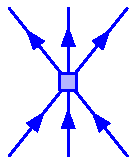
\includegraphics[width=0.5in]{figures/fig_3body_short}}
    \caption{Sources of three-body forces and the diagrams for
    their contributions in chiral effective field theory and pionless 
    EFT.}
    \label{fig:mathiot_3body}
  \end{center}
  \end{figure}



Now consider a system of three (or more nucleons).  In our low-energy effective
theory we have also eliminated degrees of freedom.
Some examples are shown in
Fig.~\ref{fig:mathiot_3body}):
       \bi
         \I excited states of nucleon, generically denoted $N^\ast$ in the figure;
         \I relativistic effects (eliminating anti-particles);
         \I integrating out high-momentum intermediate states (next week!).
       \ei
When we omit these contributions, the effects of the heavy meson exchanges are 
shrunk to points and included in a derivative expansion, as in our example
at the beginning.  If the pion is treated as a heavy degree of freedom,
it will also shrink and we will only have diagrams like the contact interaction
on the right (but with vertices with more and more powers of momentum 
or more and more derivatives, as in the two-body case).  If we resolve the
pion, we will have mid-range (middle), and long-range (left) three-body
forces, which we have characteristic spin- and isospin-dependence because
of the pion-nucleon interaction.  We will discuss the impact of such forces
on nuclear structure in later lectures.


  \begin{figure}[tbh]
  \begin{center}
    \includegraphics[width=3.8in]{figures/tjon_line_srg2}
    \caption{Tjon line: correlation of alpha particle and triton binding energies
    with different potentials.  Note where experiment lies.}
    \label{fig:tjon_line}
  \end{center}
  \end{figure}


For now, we can ask for phenomenological evidence that we will need three-body
forces.  To do so we can turn to the set of high-precision NN interactions
we discussed in an earlier lecture.  These describe the two-body physics
(nucleon-nucleon scattering and the deuteron) essentially perfectly up to
a rather high energy.  But now that us take all of the ones available and
calculate accurately the binding energies of the triton ($^3$H) and the alpha
particle ($^4$He).  If we plot the results and also the experimental point,
we find that none of the potentials agree with experiment, but interestingly 
they all lie close to a line, which is called the Tjon line
(see Fig.~\ref{fig:tjon_line}).  
To agree with experiment, for each potential we need to add a three-body
force and the energy we need is generally different in each case.
What about our expectations for 4-body and higher body?


 
\subsubsection{Three-body forces in pionless EFT}

Finally, let's return to the pionless EFT and some more formal considerations.
Feynman rules and power counting predict a three-body force is possible
and because it is allowed by the symmetries,
general EFT principles say it \emph{will} appear.
If we have only neutrons, the value is zero from the Pauli principle because
we can't have a non-zero
wave function for all three particle at the same point $\xvec$ since at least
two spins must be the same.

But when we have protons and neutrons, 
our simple perturbative case tells us we \emph{need} a three-body
contact force to fix
the contribution from our two-body interactions at high energy when
we consider the scattering of three nucleons.
At low resolution, we don't resolve a series of two-body
scatterings at high energy, 
and this implies that we need three-body, even if the underlying potential
we are trying to reproduce (e.g., hard-sphere scattering) is two-body only!
This shows up as new \emph{logarithmic} divergences in 3--3 scattering
in these diagrams:
     \beq
      \raisebox{-.2in}{\includegraphics*[width=2.2in,angle=0.0]{figures/fig_3to3}}      
           \quad   \propto {\re (C_0)^4 \ln(k/\Lambda_c)}
     \eeq
That is, if you evaluate the contribution of these Feynman diagrams, you
will find that it contains a dependence on the momentum cutoff as indicated.     
The changes in $\Lambda_c$ \emph{must} be absorbed by 
a \emph{3-body} coupling $D_0(\Lambda_c)$ where
\beq
   D_0(\Lambda_c) \propto {\re (C_0)^4 \ln (a_0\Lambda_c)}
       + \mbox{const.}
       \quad \mbox{[from Braaten \& Nieto]}
\eeq.       
   %
The requirement that the total (which is part of a measurable quantity) 
be independent of $\Lambda_c$ (which is an auxiliary parameter that must
disappear in the final result) tells us that any change with $\Lambda_c$
in the diagrams must be compensated by $D_0(\Lambda_c)$:   
  %
  \beq
    \hspace*{-.2in}
    \frac{d}{d\Lambda_c}\biggl[
    \raisebox{-.2in}{%
       \includegraphics*[width=2.4in,angle=0.0]{figures/fig_3to3b}}
    \biggr] = 0 \;,
  \eeq
and this fixes the coefficient!  This is an example of
using the \emph{renormalization group} running of a coupling
to derive new information, seemingly at no cost!



%%%%%%%%%%%%%%%%%%%%%%%%%%%%%%%%%%%%%%%%%%%%%%%%%%%%%%%%%%%%%%%%%%%%%%%%%%%%%%%%%%%%%%
%%%%%%%%%%%%%%%%%%%%%%%%%%%%%%%%%%%%%%%%%%%%%%%%%%%%%%%%%%%%%%%%%%%%%%%%%%%%%%%%%%%%%%


\end{document}


  \begin{figure}[tbh]
  \begin{center}
    \includegraphics[width=3.8in]{figures/}
    \caption{}
    \label{fig:}
  \end{center}
  \end{figure}



